\documentclass{ecnreport}

\stud{OD Robotique 2015-2016}
\topic{Examen de Middleware/ROS}

\begin{document}

\inserttitle{Examen de Middleware/ROS\newline }

\insertsubtitle{1h, documents autorisés}



\section{Initialisation de l'environnement}

\subsection{Si ROS n'est pas initialisé sur le compte}

Si votre environnement n'a pas encore été utilisé pour ROS, exécuter le script \texttt{ros\_user\_setup.sh} à télécharger depuis mon site web.
Refermez ensuite le terminal et ouvrez-en un nouveau.

\subsection{Téléchargement du package}

L'examen est téléchargeable sous forme de package ROS avec la commande suivante : 
\begin{center}\defaultstyle
\begin{lstlisting}
cd ~/ros/src
git clone https://github.com/oKermorgant/ecn_ros2015.git
\end{lstlisting}
\end{center}

\section{Description du package}

\subsection{Le simulateur}

Lancez \texttt{midwa.launch}:
\begin{center}\defaultstyle
\begin{lstlisting}
roslaunch ecn_ros2015 midwa.launch
\end{lstlisting}
\end{center}

\def\vx{v_x}
\def\wz{\omega_z}

RViz est lancé avec trois robots mobiles plans.
\begin{itemize}
 \item Un robot type BB-8 qui suit une trajectoire prédéfinie
 \item Deux robots type R2-D2 qui sont pour l'instant immobiles
\end{itemize}Ces robots évoluent en $(x,y,\theta)$ et sont commandés avec une vitesse linéaire $\vx$ et angulaire $\wz$.

\subsection{Nodes et topics}

Le node \texttt{simulator} rend compte du déplacement des trois robots. Celui de BB-8 est imposé, les autres dépendent d'une consigne de vitesse.\\
Chaque robot publie sa position sur le topic \texttt{robot\#/pose} (\texttt{\#} étant un nombre entre 1 et 3) et souscrit à une consigne de vitesse sur le topic \texttt{robot\#/cmd}.\\
Pour plus d'information, les nodes et topics sont visualisables avec \texttt{rqt\_graph} et accessibles via les commandes \texttt{rosnode} et \texttt{rostopic}.

Les topics qui nous intéressent sont :
\begin{enumerate}
 \item Les topics de position (\texttt{robot\#/pose}), sur lesquels sont publiés des messages de type \texttt{geometry\_msgs/Pose2D} dont la structure est :
 \begin{center}\defaultstyle
\begin{lstlisting}
float64 x
float64 y
float64 theta
\end{lstlisting}
\end{center}
\item Les topics de consigne (\texttt{robot\#/cmd}), sur lesquels le simulateur attend des messages de type \texttt{geometry\_msgs/Twist} de structure : 
 \begin{center}\defaultstyle
\begin{lstlisting}
geometry_msgs/Vector3 linear
  float64 x
  float64 y
  float64 z
geometry_msgs/Vector3 angular
  float64 x
  float64 y
  float64 z
\end{lstlisting}
\end{center}
\end{enumerate}

Le simulateur ne prend en compte que les champs \texttt{linear.x} (vitesse linéaire dans le repère du robot) et \texttt{angular.z} (vitesse angulaire).

\section{Objectifs}

Le travail demandé est d'écrire :
\begin{itemize}
 \item Un node qui permet à un robot d'en suivre un autre à une distance donnée
 \item Un launchfile pour exécuter deux fois le node ci-dessus, afin que les trois robots se suivent
\end{itemize}

\subsection{Écriture du node}

Le node principal est à écrire en C++\footnote{on modifiera le fichier \texttt{CMakeLists.txt} afin de le compiler}.
Créer le fichier directement dans le dossier \texttt{ecn\_midwa}.\\
Ce node doit :
\begin{enumerate}
 \item Souscrire à deux topics de pose (type \texttt{geometry\_msgs/Pose2D})
 \begin{enumerate}
  \item Le premier est nommé \texttt{current} et correspond à la pose du robot piloté
  \item Le deuxième est nommé \texttt{target} et correspond à la pose du robot visé
 \end{enumerate}
 \item Publier sur un topic de commande en vitesse (type \texttt{geometry\_msgs/Twist}), nommé \texttt{cmd}
\end{enumerate}
\newpage
Les deux poses courante $(x_c,y_c,\theta_c)$ et désirée $(x_t,y_t,\theta_t)$ sont représentées en \Fig{schema}.
\begin{figure}[h]\centering
 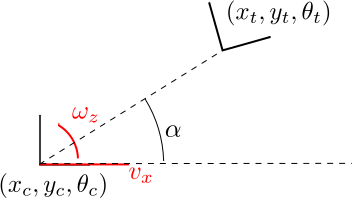
\includegraphics[width=.5\linewidth]{schema}
 \caption{Poses courante et désirée. Vitesses linéaire $\vx$ et angulaire $\omega_z$.}
 \label{schema}
\end{figure}

La loi de commande $(\vx,\wz)$ permettant au robot contrôlé de s'approcher à une distance $d$ du robot cible est calculée avec l'algorithme suivant :
\begin{enumerate}
 \item Calcul de l'erreur cartésienne entre la cible et le robot courant :
 \begin{equation*}
  \left\{\begin{array}{ll}
          dx &= x_t - x_c \\
          dy &= y_t - y_c
         \end{array}\right.
 \end{equation*}
 \item Calcul de l'erreur angulaire (à remettre dans $[-\pi,\pi]$ si besoin) :
  \begin{equation*}
  \alpha = \arctan2(dy, dx) - \theta_c
 \end{equation*}
 \item Calcul de l'erreur suivant $x$ dans le repère courant :
   \begin{equation*}
  \rho= dx\cos\theta_c + dy\sin\theta_c - d
 \end{equation*}où $d$ est la distance à laquelle on veut se placer par rapport à la cible.
 \item Loi de commande proportionnelle :
  \begin{equation*}
  \left\{\begin{array}{ll}
          \vx &= k_\rho\rho \\
          \wz &= k_\alpha \alpha
         \end{array}\right.
 \end{equation*}où $k_\rho$ et $k_\alpha$ sont des gains.
\end{enumerate}
On utilisera les valeurs suivantes pour cette application :
 \begin{equation*}
  \left\{\begin{array}{ll}
          d &= 1 \\
          k_\rho &= 2.7 \\
          k_\alpha &= 2.9
         \end{array}\right.
 \end{equation*}
La consigne $(\vx,\wz)$ est à écrire ensuite dans un message de type \texttt{geometry\_msgs/Twist} et à publier sur le topic \texttt{cmd}.
\newpage

\subsection{Écriture du launchfile}

Le node ci-dessus utilise des topics génériques, il convient donc de le lancer via un launchfile en utilisant la fonction \texttt{remap} pour l'application qui nous intéresse.\\

Écrire un launchfile permettant au robot 2 de suivre le robot 1, et au robot 3 de suivre le robot 2.\\

Pour simplifier le développement du node on pourra dans un premier temps écrire en dur les topics permettant au robot 2 de suivre le robot 1.






\end{document}